%!TEX root = ../thesis.tex
\chapter{Evaluation}
\label{ch:Evaluation}
\section{Datensammlung und Grundlage}
{ \label{sec:datengrundlage}
	Die Datengrundlage zur Analyse bilden Videos im MP4 Format in der Auflösung 1920 \texttimes 1080 Pixeln. Diese wurden an der Autobahnbrücke zur A1 in Münster-Nienberge aufgenommen \citep{GMaps}. Das Wetter war bedeckt, somit konnte die Sonne nicht einzelne Objekte überstrahlen. Das Videomaterial mit dem evaluiert wurde, stammt vom 17.07.2023 und wurde mittags (12:53 Uhr) aufgenommen. Es zeigt primär die beiden Fahrspuren der Autobahn (siehe Abb. \ref{Bsp_Evaluations_Vidmat}). \\
	Am unteren Rand ist im Vordergrund rechts das Geländer der Autobahnbrücke zu erkennen. Links unten im Bild ist ein Warnkegel zu sehen. Der mittlere Bereich des Bildes wird von den Fahrspuren dominiert, rechts mittig sind zwei Verkehrsschilder. Im Hintergrund ist ein weiteres Verkehrsschild zu erkennen, welches über die sich vom Betrachter entfernende führende Fahrspur ragt. An den Seiten der beiden Fahrspuren sind Bäume. \\
	Das Videomaterial wurde mit der Software DaVinci Resolve \citep{davinciresolve} geschnitten um die für die Evaluation wichtige Vergleichbarkeit und Frameanzahl zu erhalten.
	\begin{figure}[ht]
		\centering
		\includegraphics*[scale = 0.35, keepaspectratio ]{images/Evaluation/Screenshot_Video_A10s.png}
		\caption[Beispielframe aus Videomaterial]{Beispielframe aus Videomaterial (Quelle: eigene Darstellung)} 
		\label{Bsp_Evaluations_Vidmat}
 \end{figure}
}



\section{Einstellungen und Testdatensätze}
{% \begin{itemize}
	% 	\item Evaluation mit verschiedenen Testvideos
	% 	\item immer das gleiche Video nur mit verschiedenen Längen
	% 	\item Dann verschiedene Berechnungsmethode (YOLO every frame, yolo result)
	% 	\item mit und ohne schwarzes video ?
	% 	\item mit verschiedenen YOLO Modellen (v8n, v8x, v8)
	% \end{itemize}
	Es werden 2 Videodaten genommen, die sich jeweils in der Länge unterscheiden. Beide Testdatensätze basieren auf dem gleichen Video. Die Länge unterscheidet sich, da das erste Video 1 Sekunde, bzw. 30 Frames, lang ist und das zweite Video 10 Sekunden dauert, bzw. 300 Frames besitzt. Hier überschneidet sich die erste Sekunde. \\
	Es werden 3 YOLO Modelle benutzt: YOLO8n, YOLOv8n (small), YOLOv8m (medium) und YOLOv8x (extra large). Diese sind mit verschieden großen Datensätzen trainiert worden, für Details siehe Kapitel \ref{subsec:YOLOv8_theoretic}.
	Die Einstellungen des Programms für die Grenze der Punktsubstitution der DCE sind, dass Autos auf 8 Punkte, Motorräder auf 5 und Lkw auf 11 Punkte reduziert werden.
	% \begin{itemize}
	% 	\item Car: 10
	% 	\item Motorcycle: 5
	% 	\item Truck: 8
	% 	\item other Object: 20
	% \end{itemize}
	Objekte, welche nicht den drei Hauptklassen entsprechen werden pauschal auf 20 Punkte vereinfacht. Das Video wird  schwarz gerendert, sodass sich nur weiße Polygone im Video bewegen. Außerdem werden für jedes Polygon die detektierte Klasse und der Confidence Score in jedem Frame angezeigt.
	Der Code wird auf einem System, welches in Kap. \ref{sec:testumgebung} beschrieben wurde, ausgeführt.

}
\section{Ergebnisse\label{sec:Ergebnisse}}  

\todo{klare Benennung von YOLO oder Yolo; bzw. Yolov8n oder 8n etc.}
	\todo{Yolo Modelle ebenfalls durchgehend klar benennen}
\todo{Tabellen bei >1000 Zahlen mit 1.000 ausfüllen (Punkt zur Trennung)}
{Die Formähnlichkeit der einzelnen Polygone zueinander wird einem Messwert  (siehe Kap. \ref{theo:SSM} und \ref{py:Shape_Sim_Meas}) berechnet. Es wird zunächst auf allgemeine Erkenntnisse eingegangen und danach werden die Ergebnisse mit Klassenunterscheidung erläutert. Ein Beispielframe aus dem 10-sekündigen Datensatz ist in Abb. \ref{Bsp_ErgebRVA10s_Vidmat} zu sehen.\\
Alle Angaben in den Tabellen, außer bei den absoluten Zahlen sind in Grad (Deg.). Die Modelle von YOLO werden mit 8n, 8m, 8x entsprechend abgekürzt. Die unterschiedlichen YOLO Implementierungen werden mit EFV (Every Frame Version, 1. YOLO Implementierung) und RV (Result Version, 2. YOLO Implementierung) abgekürzt.

\todo{Bild aktualisieren}
\begin{figure}[ht]
	\centering
	\includegraphics*[scale = 0.35, keepaspectratio ]{images/Evaluation/Screenshot_A10s_RV.png}
	\caption[Beispielframe aus mit der direkten YOLO Anwendung analysiertem Videomaterial]{Beispielframe aus mit der 2. YOLO Implementierung analysiertem Videomaterial (Quelle: eigene Darstellung)} 
	\label{Bsp_ErgebRVA10s_Vidmat}
\end{figure}




\subsection{Allgemeine Erkenntnisse}
{	
	\begin{table}[h]
		\centering
		\caption[Vergleich der verschiedenen YOLO Modelle bei 10 Sekunde Video (300 Frames) (Quelle: eigene Darstellung)]{Vergleich der verschiedenen YOLO Modelle bei 10 Sekunde Video (300 Frames) (Quelle: eigene Darstellung; \ref{cd:listing_A10s_EF_results.txt(Y8n)}; \ref{cd:listing_A10s_RV_results.txt(Y8n)}; \ref{cd:listing_A10s_EF_results.txt(Y8m)}; \ref{cd:listing_A10s_RV_results.txt(Y8m)}; \ref{cd:listing_A10s_EF_results.txt(Y8x)}; \ref{cd:listing_A10s_RV_results.txt(Y8x)})}
		\label{tab:YOLO8_A10s}
		\begin{tabular}{l|l|l|l|l|l|l}
			& \textbf{8n (EFV)} & \textbf{8n (RV)} & \textbf{8m (EFV)} & \textbf{8m (RV)} & \textbf{8x (EFV)} & \textbf{8x (RV)} \\ \hline
		   \textit{\begin{tabular}[c]{@{}l@{}}Anzahl Punkte/Winkel\\ vor DCE\end{tabular}} & 54.574 & 54.565 & 59.945 & 59.908 & 57.753 & 57.673 \\ \hline
		   \textit{\begin{tabular}[c]{@{}l@{}}Anzahl Punkte/Winkel\\ nach DCE\end{tabular}} & 17.300 & 17.298 & 20.571 & 20.575 & 20.164 & 20.132 \\ \hline
		   \textit{\begin{tabular}[c]{@{}l@{}}Anzahl vergl. Winkel\\ bei SSM Berechnung\end{tabular}} & 104.128 & 102.718 & 103.275 & 102.962 & 120.091 & 119.714 \\ \hline
		   \textit{} &  &  &  &  &  &  \\ \hline
		   \textit{\begin{tabular}[c]{@{}l@{}}Gesamtwinkelsumme\\ (in Deg.)\end{tabular}} & 54.307,46 & 54.301,23 & 64.559,41 & 64.571,89 & 63.273,38 & 63.172,79 \\ \hline
		   \textit{erk.  Polygone} & 1.377 & 1.376 & 2.021 & 2.020 & 2.108 & 2.104 \\ \hline
		   \textit{verglichene Polygone} & 1.235 & 1.234 & 1.871 & 1.870 & 1.964 & 1960 \\ \hline
		   \textit{\begin{tabular}[c]{@{}l@{}}Prozessierungszeit\\ (in Min.)\end{tabular}} & 5,46 & 4,1 & 9,11 & 5,85 & 14,94 & 7,99
		   \end{tabular}
	\end{table}
	In Tabelle \ref{tab:YOLO8_A10s} sind allgemeine Daten zur den Testdurchläufen bei dem 10-sekündigen Testdatensatz dargestellt. Es wird zunächst auf allgemeine Erkenntnisse eingegangen, da die beiden verschiedenen YOLO Implementierungen sich nur marginal unterscheiden. Die Tabelle \ref{tab:YOLO8_A1s} zeigt die Ergebnisse für den 1-sekündigen Testdatensatz. Diese Ergebnisse sind ähnlich zu den im Folgenden beschriebenen, außer das die Zahlen und Ergebnisse deutlich kleiner sind. 
	Wenn man die verschiedenen YOLO Modelle im Bereich der Punktzahlen vor der Vereinfachung mit der DCE betrachtet, ist auffällig, dass diese Zahlen relativ konstant bleiben. Es ist jedoch ein kleiner Anstieg bei Verwendung der mit mehr Testdaten trainierten Modell zu erkennen. Insbesondere ist ein  Unterschied von ca. 4.000 Punkten zwischen 8n und 8m vorhanden, während die Punktzahl im Vergleich von 8m zu 8x um ca. 2.000 Punkte sinkt. \\
	Wenn man nun die Anzahl der Punkte nach der Vereinfachung betrachtet, ist auch hier ein kleiner Anstieg zwischen 8n und 8m zu erkennen, auch wenn die Zahlen von 8m und 8x im Vergleich sehr konstant sind. Der Unterschied beim Anstieg von 8n zu 8m beträgt ungefähr 3.000 Punkte. 
	Die Anzahl der verglichenen Winkel ist deutlich höher, als die Punktanzahl. Diese Zahlen sind mit ca. 100.000 Vergleichen um das ca. 5-fache höher als überhaupt Punkte nach der Vereinfachung vorhanden sind. Es ist auffällig, dass die Zahlen zwischen 8n und 8m relativ konstant sind, während die Vergleichsanzahl bei 8x um ca. 20.000 Punkte ansteigt.\\
	Bei der Zahl der verglichenen und erkannten Polygone ist ein Anstieg bei der Verwendung des besseren YOLO Modelles erkennbar. Dieser Anstieg ist insbesondere zwischen 8n und 8m mit ca. 700 Polygonen bei der Polygongesamtanzahl sehr ausgeprägt, während die Zahlen beim Vergleich von 8m und 8x relativ konstant bleiben, bzw. der Anstieg mit ca. 100 Polygonen sehr viel geringer vorhanden ist. Ein ähnliches Phänomen ist bei der Anzahl der verglichenen Polygone erkennbar, hier ist der Anstieg von 8n zu 8m mit ca. 600 Polygonen geringer als bei der Gesamtanzahl der Polygone. Jedoch ist auch hier ein minimaler Anstieg von ca. 100 Polygonen im Vergleich von 8m zu 8x zu erkennen.\\
	Bei der Prozessierungszeit ist einer der wenigen Unterschiede bei den verschiedenen Implementierung von YOLO zu erkennen. Bei dem kleinsten YOLO Modell 8n ist der Unterschied zwischen EFV und RV mit ca. 1 Minute noch sehr gering, während er bei Verwendung des mittleren YOLO Modell mit ca. 4 Minuten ausgeprägter ist. Bei der Verwendung des größten YOLO Modells kann die Rechenzeit mit der RV Version fast halbiert werden im Vergleich zu der EV Version. Der Unterschied beträgt hier ca. 7 Minuten. 

	\begin{table}[h]
		\centering
	\caption[Vergleich der verschiedenen YOLO Modelle bei 1 Sekunde Video (30 Frames) (Quelle: eigene Darstellung)]{Vergleich der verschiedenen YOLO Modelle bei 1 Sekunde Video (30 Frames) (Quelle: eigene Darstellung; \ref{cd:listing_A1s_EF_results.txt(Y8n)}; \ref{cd:listing_A1s_RV_results.txt(Y8n)}; \ref{cd:listing_A1s_EF_results.txt(Y8m)}; \ref{cd:listing_A1s_RV_results.txt(Y8m)}; \ref{cd:listing_A1s_EF_results.txt(Y8x)}; \ref{cd:listing_A1s_RV_results.txt(Y8x)})}
	\label{tab:YOLO8_A1s}
	\begin{tabular}{l|l|l|l|l|l|l}
		& \textbf{8n (EFV)} & \textbf{8n (RV)} & \textbf{8m (EFV)} & \textbf{8m (RV)} & \textbf{8x (EFV)} & \textbf{8x (RV)} \\ \hline
	\textit{\begin{tabular}[c]{@{}l@{}}Anzahl Punkte/Winkel\\ vor DCE\end{tabular}} & 5.353 & 5.303 & 5.863 & 5.885 & 5.306 & 5.325 \\ \hline
	\textit{\begin{tabular}[c]{@{}l@{}}Anzahl Punkte/Winkel\\ nach DCE\end{tabular}} & 1.919 & 1.880 & 2.168 & 2.185 & 1.965 & 1.988 \\ \hline
	\textit{\begin{tabular}[c]{@{}l@{}}Anzahl vergl. Winkel\\ bei SSM Berechnung\end{tabular}} & 19.100 & 17.811 & 10.251 & 10.130 & 11.803 & 11.858 \\ \hline
	\textit{} &  &  &  &  &  &  \\ \hline
	\textit{\begin{tabular}[c]{@{}l@{}}Gesamtwinkelsumme\\ (in Deg.)\end{tabular}} & 6.020,32 & 5.898,2 & 6.802,79 & 6.856,27 & 6.166,18 & 6.238,21 \\ \hline
	\textit{erkannte Polygone} & 147 & 145 & 209 & 210 & 212 & 214 \\ \hline
	\textit{verglichene Polygone} & 131 & 129 & 188 & 189 & 193 & 194 \\ \hline
	\textit{Prozessierungszeit (in Sek.)} & 29,54 & 20,19 & 47,92 & 30.64 & 80,15 & 44,09
	\end{tabular}
	\end{table}
}





\subsection{Formähnlichkeitsmesswert}

	
\begin{table}[h]
	\caption{Vergleich der SSMs bei verschiedenen YOLO8 bei 10 Sekunde Video (300 Frames)}
	\label{tab:YOLO8_A10s_SSM}
	\begin{tabular}{l|l|l|l|l|l|l}
	 & \textbf{8n (EFV)} & \textbf{8n (RV)} & \textbf{8m (EFV)} & \textbf{8m (RV)} & \textbf{8x (EFV)} & \textbf{8x (RV)} \\ \hline
	\textit{Absolute SSM Auto} & 39,7962 & 39,7962 & 51,9478 & 51,9478 & 58,6034 & 58,6721 \\ \hline
	\textit{SSM pro Fr. und Kl. Auto} & 0,1327 & 0,1327 & 0,1732 & 0,1732 & 0,1953 & 0,1956 \\ \hline
	\textit{SSM pro detektiertes Auto} & 0,1618 & 0,1631 & 0,1234 & 0,1243 & 0,1112 & 0,1118 \\ \hline
	\textit{\begin{tabular}[c]{@{}l@{}}absolute Anz. detektierter\\ Autos (in Klam. pro Fr.)\end{tabular}} & \begin{tabular}[c]{@{}l@{}}246 \\ (0,82)\end{tabular} & \begin{tabular}[c]{@{}l@{}}244 \\ (0,81)\end{tabular} & \begin{tabular}[c]{@{}l@{}}421\\ (1,4)\end{tabular} & \begin{tabular}[c]{@{}l@{}}418\\ (1,39)\end{tabular} & \begin{tabular}[c]{@{}l@{}}527\\ (1,76)\end{tabular} & \begin{tabular}[c]{@{}l@{}}525\\ (1,7)\end{tabular} \\ \hline
	 &  &  &  &  &  &  \\ \hline
	\textit{Absolute SSM LKW} & 70,9389 & 70,9389 & 147,2899 & 147,5313 & 154,1550 & 154,1550 \\ \hline
	\textit{SSM pro Fr. und Kl. LKW} & 0,2365 & 0,2365 & 0,4910 & 0,4918 & 0,5138 & 0,5147 \\ \hline
	\textit{SSM pro detektierter LKW} & 0,3657 & 0,3676 & 0,2683 & 0,2692 & 0,2120 & 0,2127 \\ \hline
	\textit{\begin{tabular}[c]{@{}l@{}}absolute Anz. detektierter\\ LKW (in Klam. pro Fr.)\end{tabular}} & \begin{tabular}[c]{@{}l@{}}194\\ (0,65)\end{tabular} & \begin{tabular}[c]{@{}l@{}}193\\ (0,64)\end{tabular} & \begin{tabular}[c]{@{}l@{}}549\\ (1,83)\end{tabular} & \begin{tabular}[c]{@{}l@{}}548\\ (1,83)\end{tabular} & \begin{tabular}[c]{@{}l@{}}727\\ (2,42)\end{tabular} & \begin{tabular}[c]{@{}l@{}}726\\ (2,42)\end{tabular} \\ \hline
	 &  &  &  &  &  &  \\ \hline
	\textit{Absolute SSM Zug} & 34,2706 & 34,2706 & 8,2767 & 8,2767 & 1,9969 & 1,9969 \\ \hline
	\textit{SSM pro Fr. und Kl. Zug} & 0,1142 & 0,1142 & 0,0276 & 0,0276 & 0,0067 & 0,0067 \\ \hline
	\textit{SSM pro detektierten Zug} & 0,3808 & 0,3939 & 1,6553 & 1,6553 & 1,9969 & 1,9969 \\ \hline
	\textit{\begin{tabular}[c]{@{}l@{}}absolute Anz. detektierter\\ Züge (in Klam. pro Fr.)\end{tabular}} & \begin{tabular}[c]{@{}l@{}}90\\ (0,3)\end{tabular} & \begin{tabular}[c]{@{}l@{}}87\\ (0,29)\end{tabular} & \begin{tabular}[c]{@{}l@{}}5\\ (0,02)\end{tabular} & \begin{tabular}[c]{@{}l@{}}5\\ (0,02)\end{tabular} & \begin{tabular}[c]{@{}l@{}}1\\ (0,00)\end{tabular} & \begin{tabular}[c]{@{}l@{}}1\\ (0,00)\end{tabular} \\ \hline
	 &  &  &  &  &  &  \\ \hline
	\textit{Absolute SSM Bus} & 3,7216 & 3,7216 & 3,9062 & 3,9062 &  &  \\ \hline
	\textit{SSM pro Fr. und Kl. Bus} & 0,0124 & 0,0124 & 0,013 & 0,013 &  &  \\ \hline
	\textit{SSM pro detektiertem Bus} & 0,3101 & 0,3101 & 0,3551 & 0,3551 &  &  \\ \hline
	\textit{\begin{tabular}[c]{@{}l@{}}absolute Anz. detektierter\\ Busse (in Klam. pro Fr.)\end{tabular}} & \begin{tabular}[c]{@{}l@{}}12\\ (0,04)\end{tabular} & \begin{tabular}[c]{@{}l@{}}12\\ (0,04)\end{tabular} & \begin{tabular}[c]{@{}l@{}}11\\ (0,04)\end{tabular} & \begin{tabular}[c]{@{}l@{}}11\\ (0,04)\end{tabular} &  & 
	\end{tabular}
	\end{table}
	Es wird nun auf die Tabelle \ref{tab:YOLO8_A10s_SSM} mit dem 10-sekündigen Testdatensatz eingegangen. Bei dem 1-sekündigen Testdatensatz sind ähnliche Effekte bei geringeren Werten zu erkennen. \\
	Wenn man beide Implementierungen von YOLO vergleicht, sieht man bei den SSM Werten ebenfalls, dass der Unterschied nur marginal ist. Aus diesem Grund wird im folgenden kein dedizierter Vergleich zwischen den Implementierungen stattfinden. \\
	Wenn man den Absolutbetrag der SSM betrachtet, sieht man bei der Klasse Auto eine Steigerung im Vergleich von 8n zu 8m. Diese Steigerung ist auch bei 8m und 8x in geringerem Ausmaß vorhanden. Bei der Abweichung pro Frame und Klasse Auto sind diese Effekte in abgeschwächter Form ebenfalls vorhanden. Hingegen ist bei der SSM pro Auto eine Verringerung bei größer werdendem Modell zu erkennen. Diese Verringerung ist besonders zwischen 8n und 8m zu erkennen, während zwischen 8m und 8x der Unterschied nur marginal ist. \\
	Bei der absoluten Anzahl detektierter Autos ist fast eine Verdoppelung zwischen 8n und 8m vorhanden. Zwischen 8m und 8x ist die Steigerung mit ca. 100 geringer ausgeprägt. \\
	Beim Absolutbetrag der SSM bei der Klasse LKW ist eine Verdoppelung zwischen den Modellen 8n und 8m zu sehen, während der Anstieg zwischen 8m und 8x deutlich geringer ausfällt. Ähnliche Effekte sind auch bei der SSM pro Frame und Klasse LKW, der SSM pro detektiertem LKW und der absoluten Anzahl detektierter LKW zu sehen. \\
	Bei der Klasse Zug ist hingegen eine deutliche Verringerung der absoluten SSM vorhanden. Dies betrifft auch die SSM pro Frame und Klasse Zug, während die SSM pro detektiertem Zug in geringem Maße bei bessere Modell von 8n zu 8x weiter ansteigt. Besonders ist jedoch die starke Reduzierung der absoluten Anzahl von Zügen zwischen 8n und 8m von 87 auf 5 und der noch weiteren Verringerung bei der Verwendung von 8x auf 1. \\
	Bei der Klasse Bus sind ähnliche Effekte wie bei der Klasse Zug zu beobachten. Besonders ist hier, dass diese Klasse von 8x nicht mehr detektiert wird und damit auch keine Werte für diese Klasse vorhanden sind.

	\begin{table}[]
		\caption{Vergleich der SSMs bei verschiedenen YOLO8 bei 1 Sekunde Video (30 Frames)}
		\label{tab:YOLO8_A1s_SSM}
		\begin{tabular}{l|l|l|l|l|l|l}
		 & \textbf{8n (EFV)} & \textbf{8n (RV)} & \textbf{8m (EFV)} & \textbf{8m (RV)} & \textbf{8x (EFV)} & \textbf{8x (RV)} \\ \hline
		\textit{Absolute SSM Auto} & 2,0174 & 2,0174 & 2,2393 & 2,3659 & 3,8058 & 4,1018 \\ \hline
		\textit{SSM pro Fr. und Kl. Auto} & 0,0672 & 0,0672 & 0,0746 & 0,0789 & 0,1269 & 0,1637 \\ \hline
		\textit{SSM pro detektiertes Auto} & 0,0672 & 0,0721 & 0,0622 & 0,0676 & 0,0634 & 0,0672 \\ \hline
		\textit{\begin{tabular}[c]{@{}l@{}}absolute Anz. detektierter\\ Autos (in Klam. pro Fr.)\end{tabular}} & \begin{tabular}[c]{@{}l@{}}30\\ (1,00)\end{tabular} & \begin{tabular}[c]{@{}l@{}}28\\ (0,93)\end{tabular} & \begin{tabular}[c]{@{}l@{}}36\\ (1,2)\end{tabular} & \begin{tabular}[c]{@{}l@{}}35\\ (1,17)\end{tabular} & \begin{tabular}[c]{@{}l@{}}60\\ (2,00)\end{tabular} & \begin{tabular}[c]{@{}l@{}}61\\ (2,23)\end{tabular} \\ \hline
		 &  &  &  &  &  &  \\ \hline
		\textit{Absolute SSM LKW} & 4,4640 & 4,6617 & 13,3996 & 14,2144 & 11,5296 & 11,8367 \\ \hline
		\textit{SSM pro Fr. und Kl. LKW} & 0,1488 & 0,1554 & 0,4467 & 0,4738 & 0,3843 & 0,3946 \\ \hline
		\textit{SSM pro detektierter LKW} & 0,2349 & 0,2454 & 0,2197 & 0,2330 & 0,1696 & 0,1767 \\ \hline
		\textit{\begin{tabular}[c]{@{}l@{}}absolute Anz. detektierter\\ LKW (in Klam. pro Fr.)\end{tabular}} & \begin{tabular}[c]{@{}l@{}}19\\ (0,63)\end{tabular} & \begin{tabular}[c]{@{}l@{}}19\\ (0,63)\end{tabular} & \begin{tabular}[c]{@{}l@{}}61\\ (2,03)\end{tabular} & \begin{tabular}[c]{@{}l@{}}61\\ (2,03)\end{tabular} & \begin{tabular}[c]{@{}l@{}}68\\ (2,27)\end{tabular} & \begin{tabular}[c]{@{}l@{}}67\\ (2,23)\end{tabular} \\ \hline
		 &  &  &  &  &  &  \\ \hline
		\textit{Absolute SSM Zug} & 11,8231 & 11,8231 &  &  &  &  \\ \hline
		\textit{SSM pro Fr. und Kl. Zug} & 0,3941 & 0,3941 &  &  &  &  \\ \hline
		\textit{SSM pro detektierten Zug} & 0,3111 & 0,3378 &  &  &  &  \\ \hline
		\textit{\begin{tabular}[c]{@{}l@{}}absolute Anz. detektierter\\ Züge (in Klam. pro Fr.)\end{tabular}} & \begin{tabular}[c]{@{}l@{}}38\\ (1,27)\end{tabular} & \begin{tabular}[c]{@{}l@{}}35\\ (1,17)\end{tabular} &  &  &  &  \\ \hline
		 &  &  &  &  &  &  \\ \hline
		\textit{Absolute SSM Bus} &  &  & 1,8576 & 1,8576 &  &  \\ \hline
		\textit{SSM pro Fr. und Kl. Bus} &  &  & 0,0619 & 0,0619 &  &  \\ \hline
		\textit{SSM pro detektiertem Bus} &  &  & 0,4644 & 0,4644 &  &  \\ \hline
		\textit{\begin{tabular}[c]{@{}l@{}}absolute Anz. detektierter\\ Busse (in Klam. pro Fr.)\end{tabular}} &  &  & \begin{tabular}[c]{@{}l@{}}4\\ (0,13)\end{tabular} & \begin{tabular}[c]{@{}l@{}}4\\ (0,13)\end{tabular} &  & 
		\end{tabular}
		\end{table}

	
} 
%\clearpage
	

\section{weitere Testfälle}
{
	In diesem Abschnitt werden weitere Testfälle thematisiert, die andere Aspekte der Software abdecken. Es werden andere Einstellungen und Testdatensätze genutzt, deren Einzelheiten in den jeweiligen Abschnitten erläutert werden.

}
\subsection{Schiffstracking \label{ev:shiptracking}}
{ 
	Dieser Testdatensatz enthält zwei Schiffe, die auf der Elbe im Hamburg zu sehen sind. Das Wetter ist nicht bedeckt und das Video wurde morgens aufgenommen. Es sind zwei verschiedene Testdatensätze aus einem Video geschnitten worden. Der kurze Testdatensatz hat 30 Frames und 1 Sekunde Länge, der lange Testdatensatz ist das ungeschnittene Video mit 642 Frames und 21 Sekunden Länge. Für ein Beispielframe aus dem Testdatensatz und dem analysiertem Datensatz siehe Abb. \ref{Scr:Testdatensatz_Shiptracking}. Hier fällt auf das die Qualität des Videos trotz der hohen Auflösung von 1920 \texttimes 1080 Pixeln durch die hohe Zoomstufe gering ist. Außerdem ist eine Boje mittig im Bild und verdeckt teilweise ein fahrendes Schiff. \\
	Die Einstellungen des Programmes wurden abgeändert, sodass das gesamte Video nicht mehr schwarz gefärbt wird, sondern nur die erkannten Boundingboxen der Objekte, wo jedoch die Umrisse weiß gezeichnet werden. Außerdem wurde der DCE Substitutionswert für andere Objekte auf 20 Punkte gesetzt, da die Klasse \glqq Boat\grqq{} unter diese Einordnung fällt. Es wurde immer das 8x Modell von YOLO benutzt. \\

		\todo{Bild muss noch aktualisiert werden}
	\begin{figure}[ht]
		\centering
		\begin{subfigure}[b]{0.45\textwidth}
			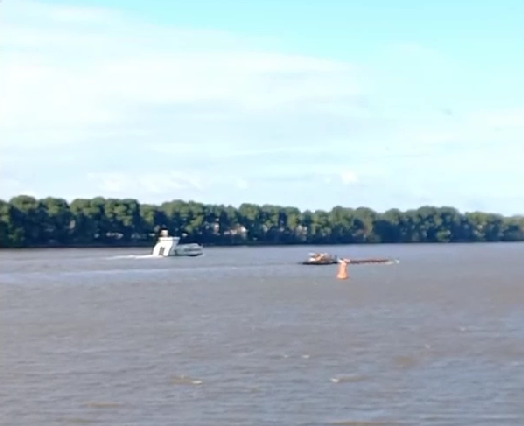
\includegraphics[width=\textwidth]{images/Evaluation/shiptracking_raw.png}
			\caption{Screenshot aus Beispieldatensatz Schiffstracking}
		\end{subfigure} \hfill
		\begin{subfigure}[b]{0.45\textwidth}
			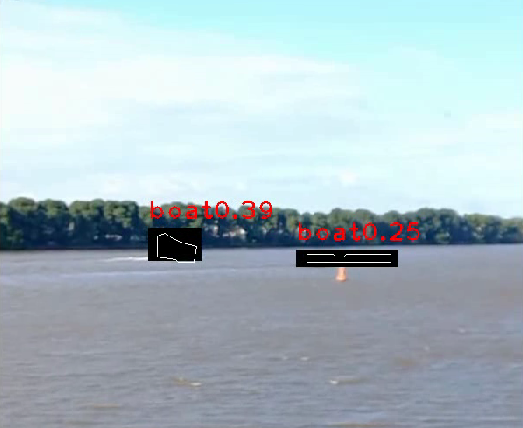
\includegraphics[width=\textwidth]{images/Evaluation/shiptracking_analyzed.png}
			\caption{Screenshot aus analysiertem Beispieldatensatz Schiffstracking}
		\end{subfigure}
		\caption[Screenshots zu Testdatensatz für Schiffstracking]{Screenshots zu Testdatensatz für Schiffstracking. (a) zeigt die Testdaten ohne Bearbeitung; (b) zeigt den Frame mit YOLO analysiert und von der DCE vereinfacht (Quelle: eigene Darstellung)}
		\label{Scr:Testdatensatz_Shiptracking}
	\end{figure} 
	Die Ergebnisse der statistischen Auswertung (s. Tabelle \ref{tab:Shiptracking_Analysis}) zeigen steigende Werte in fast allen Bereichen. Die Anzahl der Punkte vor und nach DCE steigt um das ca. 26-fache im Vergleich zwischen den Videolängen an. Die Anzahl der verglichenen Winkel steigt um mehr als das 200-fache, während die Gesamtwinkelsumme wieder um den Faktor 26  ansteigt. Die Zahl der erkannten Polygone steigt hingegen nicht so stark an (ca. Faktor 22), wie die Zahl der verglichenen Polygone (ca. Faktor 25). \\
	Bei der Prozessierungszeit ist eine Steigerung um den Faktor 22 zu erkennen, während YOLO den größten Teil davon mit 31,51 Sekunden bei dem 1-sekündigem Testdatensatz, bzw. 706,76 Sekunden (11,33 Minuten) bei dem 21-sekündigem Testdatensatz ausmacht. Die DCE hat mit 0,15 Millisekunden (bzw. 19,62 Millisekunden) einen sehr geringen Anteil an der Laufzeit bei diesen Testdatensätzen, jedoch ist hier der Faktor für den Anstieg zwischen den Videos mit ca. 130 sehr hoch. \\
	Bei der SSM ist der absolute Anstieg zwischen den Videos bemerkenswert, da dieser von ca. 2 auf ca. 150 wächst und damit ungefähr um den Faktor 80 ansteigt. Der SSM pro Frame und Klasse Boot sinkt hingegen, während die Anzahl erkannter Boote massiv um den Faktor 12 (von 46 auf 1212 detektierten Booten auf allen Frames) ansteigt. Letzteres ist auch bei der Zahl der erkannten Boote pro Frame zu erkennen. \\

	\begin{table}[]
		\centering
		\caption[Auswertung Schiffstracking Datensatz]{Auswertung Schiffstracking Datensatz; S1s ist der 1-sekündige Datensatz, S21s ist der 21-sekündige Datensatz (Quelle: eigene Darstellung; \ref{cd:listing_A1s_RV_shiptracking_results.txt(Y8x)}, \ref{cd:listing_A21s_RV_shiptracking_results.txt(Y8x)})}
		\label{tab:Shiptracking_Analysis}
		\begin{tabular}{l|l|l|l}
			& \textbf{S1s\_Y8x} & \textbf{S21s\_Y8x} & \textbf{Faktor} \\ \hline
		   \textit{\begin{tabular}[c]{@{}l@{}}Anzahl Punkte/Winkel\\ vor DCE\end{tabular}} & 763 & 22.093 & 28,96 \\ \hline
		   \textit{\begin{tabular}[c]{@{}l@{}}Anzahl Punkte/Winkel\\ nach DCE\end{tabular}} & 762 & 19.874 & 26,08 \\ \hline
		   \textit{\begin{tabular}[c]{@{}l@{}}Anzahl vergl. Winkel\\ bei SSM Berechnung\end{tabular}} & 1.380 & 286.468 & 207,59 \\ \hline
			&  &  &  \\ \hline
		   \textit{Gesamtwinkelsumme} & 2392.73 & 62.363,07 & 26,06 \\ \hline
		   \textit{erk. Polygone} & 60 & 1.310 & 21,83 \\ \hline
		   \textit{vergl. Polygone} & 49 & 1.213 & 24,76 \\ \hline
			&  &  &  \\ \hline
		   \textit{\begin{tabular}[c]{@{}l@{}}Prozessierungszeit \\ (in Sek.)\end{tabular}} & 31,51 & \begin{tabular}[c]{@{}l@{}}706,76\\ (11,78 Min.)\end{tabular} & 22,79 \\ \hline
		   \textit{Dauer YOLO (in Sek.)} & 34,51 & \begin{tabular}[c]{@{}l@{}}679,66\\ (11,33 Min.)\end{tabular} & 19,69 \\ \hline
		   \textit{Dauer DCE (in ms.)} & 0,15 & 19,62 & 129,46 \\ \hline
			&  &  &  \\ \hline
		   \textit{Absolute SSM Boot} & 1,9636 & 151,1244 & 79,96 \\ \hline
		   \textit{SSM pro Fr. und Kl. Boot} & 0,0655 & 0,2354 & 3,59 \\ \hline
		   \textit{SSM pro detektierten Boot} & 0,427 & 0,1246 & 0,27 \\ \hline
		   \textit{\begin{tabular}[c]{@{}l@{}}absolute Anz. detektierter\\ Boote (in Klam. pro Fr.)\end{tabular}} & \begin{tabular}[c]{@{}l@{}}46\\ (1,53)\end{tabular} & \begin{tabular}[c]{@{}l@{}}1212\\ (1,89)\end{tabular} & \begin{tabular}[c]{@{}l@{}}12,35\\ (1,24)\end{tabular}
		   \end{tabular}
		\end{table}

	
       \todo{Abschluss finden?}



}
\subsection{Geringe und hohe DCE Substitution (NICHT FERTIG)} \todo{ab hier muss noch text überarbeitet/geschrieben werden}
	{ \todo{tabelen mit quellen versehen!}
		Bei diesem Testdaten werden die Fälle betrachtet, bei denen DCE geringere und höhere Punktgrenzen beachten muss. Als Referenz wird der 8x Datensatz in der Länge 1 Sekunde und in der Länge 10 Sekunden genutzt. Es wird immer die RV Version der Implementierung mit dem YOLOv8x Modell betrachtet. Die DCE Grenzen sind in Tabelle \ref{tab:YOLO8_minor_more_DCE_Limits} aufgelistet. Der SSM wird aufgrund von nur kleineren Unterschieden bei den anderen Klassen anhand der beiden Hauptklassen Auto und LKW beurteilt. \\
		Im Folgenden wird sich auf den 10-sekündigen Testdatensatz bezogen, da die Ergebnisse auf den 1-sekündigen Datensatz übertragbar sind. Hier ist die einzige Besonderheit das alle Werte deutlich geringer sind (siehe Tabelle \ref{tab:YOLO8_minor_more_DCE_A1s}, S. \pageref{tab:YOLO8_minor_more_DCE_A1s}  und Tabelle \ref{tab:Minor_More_DCE_SSMs_A1s}, S. \pageref{tab:Minor_More_DCE_SSMs_A1s}). \\
	\begin{table}[ht]
		\caption{Einstellungen der verschiedenen DCE Substitutionsgrenzen (Quelle: eigene Darstellung; \ref{cd:listing_A1s_RV_minor_results.txt(Y8x)}, \ref{cd:listing_A1s_RV_more_results.txt(Y8x)}, \ref{cd:listing_A10s_RV_minor_results.txt(Y8x)}, \ref{cd:listing_A10s_RV_more_results.txt(Y8x)})}
		\label{tab:YOLO8_minor_more_DCE_Limits}
		\centering
		\begin{tabular}{l|l|l|l}
		 & \textbf{\begin{tabular}[c]{@{}l@{}}geringe DCE\\ Punktgrenzen\end{tabular}} & \textbf{Referenz} & \textbf{\begin{tabular}[c]{@{}l@{}}hohe DCE\\ Punktgrenzen\end{tabular}} \\ \hline
		\textit{Kl. Auto} & 5 & 8 & 60 \\ \hline
		\textit{Kl. Motorrad} & 3 & 5 & 25 \\ \hline
		\textit{Kl. LKW} & 6 & 11 & 40 \\ \hline
		\textit{anderes Objekt} & 5 & 20 & 100
		\end{tabular}
		\end{table} In Tabelle \ref{tab:YOLO8_minor_more_DCE_A10s} ist zu sehen, dass die Punktanzahl vor der DCE Vereinfachung bei allen drei Testdurchläufen exakt gleich gewesen ist. Ein Unterschied ist bei der Anzahl der Punkte nach dem Durchlauf der DCE zu erkennen, da bei der geringen Punktgrenze ein niedriger Wert und bei der hohen Punktgrenze ein höherer Wert als beim Referenzdatensatz gemessen wurde. Die Anzahl der verglichenen Winkel steigt im Vergleich zwischen allen drei Durchläufen stark an. \\
		Dieser starke Anstieg ist auch bei der Gesamtwinkelsumme zu erkennen. Die erkannten und verglichenen Polygone bleiben hingegen über alle 3 Testdurchläufe exakt gleich. \\
		Bei der Dauer der Prozessierung ist eine geringe Verbesserung zu einer kürzeren Dauer zu erkennen.\\

		
	
			\begin{table}[ht]
				\caption{Vergleich der Statistik bei 10 Sekunde Video (300 Frames) und verschiedenen DCE Substitutionsgrenzen (Quelle: eigene Darstellung; \ref{cd:listing_A10s_RV_minor_results.txt(Y8x)}, \ref{cd:listing_A10s_RV_more_results.txt(Y8x)})}
				\label{tab:YOLO8_minor_more_DCE_A10s}
				\centering
				\begin{tabular}{l|l|l|l}
					& \textbf{\begin{tabular}[c]{@{}l@{}}geringe DCE\\ Punktgrenzen\end{tabular}} & \textbf{Referenz} & \textbf{\begin{tabular}[c]{@{}l@{}}hohe DCE\\ Punktgrenzen\end{tabular}} \\ \hline
				   \textit{\begin{tabular}[c]{@{}l@{}}Anzahl Punkte/Winkel \\ vor DCE\end{tabular}} & 57.673 & 57.673 & 57.673 \\ \hline
				   \textit{\begin{tabular}[c]{@{}l@{}}Anzahl Punkte/Winkel\\ nach DCE\end{tabular}} & 11.584 & 20.132 & 43.040 \\ \hline
				   \textit{\begin{tabular}[c]{@{}l@{}}Anzahl vergl. Winkel\\ bei SSM Berechnung\end{tabular}} & 39.703 & 119.714 & 769.311 \\ \hline
				   \textit{} &  &  &  \\ \hline
				   \textit{Gesamtwinkelsumme} & 36.389,37 & 63.172,79 & 135.064,50 \\ \hline
				   \textit{erkannte Polygone} & 2.104 & 2.104 & 2.104 \\ \hline
				   \textit{verglichene Polygone} & 1.960 & 1.960 & 1.960 \\ \hline
				   \textit{Prozessierungszeit (in Min.)} & 8,48 & 7,99 & 7,22
				   \end{tabular}
				\end{table}

				Bei der SSM von den Klassen Auto und LKW (s. Tabelle \ref{tab:Minor_More_DCE_SSMs_A10s}) sind ähnliche Effekte zu sehen. Die absolute Abweichung bei der Klasse Auto, wie auch bei der Klasse LKW steigt um mehr als das Doppelte im Vergleich von dem geringen zum hohen DCE Substitionslimit. Den gleichen Effekt kann man auch der SSM pro Frame und Klasse Auto oder LKW und bei der SSM pro detektiertem Auto oder LKW sehen. Die absolute Anzahl Auto und LKW (auch pro Frame) bleibt hingegen über alle drei Testfälle exakt gleich.	
	
				\begin{table}[ht]
					\caption{Vergleich der SSMs bei verschiedenen DCE Substitionslimits bei einem 10-sekündigem Video (300 Frames) (Quelle: eigene Darstellung; \ref{cd:listing_A10s_RV_minor_results.txt(Y8x)}, \ref{cd:listing_A10s_RV_more_results.txt(Y8x)})}
					\label{tab:Minor_More_DCE_SSMs_A10s}
					\centering
					\begin{tabular}{l|l|l|l}
						& \textbf{\begin{tabular}[c]{@{}l@{}}geringe DCE\\ Punktgrenzen\end{tabular}} & \textbf{Referenz} & \textbf{\begin{tabular}[c]{@{}l@{}}hohe DCE\\ Punktgrenzen\end{tabular}} \\ \hline
					   \textit{Absolute SSM Auto} & 43,438 & 58,6721 & 97,1323 \\ \hline
					   \textit{SSM pro Fr. und Kl. Auto} & 0,1448 & 0,1956 & 0,3238 \\ \hline
					   \textit{SSM pro detektiertes Auto} & 0,0827 & 0,1118 & 0,1850 \\ \hline
					   \textit{\begin{tabular}[c]{@{}l@{}}absolute Anz. detektierter\\ Autos (in Kl. pr. Fr.)\end{tabular}} & \begin{tabular}[c]{@{}l@{}}525\\ (1,75)\end{tabular} & \begin{tabular}[c]{@{}l@{}}525\\ (1,75)\end{tabular} & \begin{tabular}[c]{@{}l@{}}525\\ (1,75)\end{tabular} \\ \hline
					   \textit{} &  &  &  \\ \hline
					   \textit{Absolute SSM LKW} & 112,7181 & 154,3962 & 255,6707 \\ \hline
					   \textit{SSM pro Fr. und Kl. LKW} & 0,3757 & 0,5147 & 0,8522 \\ \hline
					   \textit{SSM pro detektierten LKW} & 0,1553 & 0,2127 & 0,3522 \\ \hline
					   \textit{\begin{tabular}[c]{@{}l@{}}Absolute Anz. detektierter\\ LKW (in Kl. pro Fr.)\end{tabular}} & \begin{tabular}[c]{@{}l@{}}726\\ (2,42)\end{tabular} & \begin{tabular}[c]{@{}l@{}}726\\ (2,42)\end{tabular} & \begin{tabular}[c]{@{}l@{}}726\\ (2,42)\end{tabular}
					   \end{tabular}
					\end{table}
		
	}
	 \clearpage
\subsection{lange Testdatensätze (NICHT FERTIG)}{
	\todo{müssen noch gemacht werden }
	
}
\subsection{Gleiche DCE Substitionslimits (NICHT FERTIG)}{
	\todo{müssen noch gemacht werden }}
{
	

}
% 	\section{Bewertung}
% 	{ %Zusammenfassen kann man sagen, dass die durchschnittliche Abweichung pro Polygon nach der Vereinfachung von DCE zu hoch ist, um ein Tracking zu ermöglichen. Beim Einsatz der größeren Modelle steigt die Winkelabweichung und SSM an, dies ist aber zu vernachlässigen, da die Klassifizierung der Objekte genauer erfolgt. Insbesondere der Vergleich der SSM innerhalb einer Klasse  ist die Abweichung sehr hoch. \\
% 	%Die Implementierung der YOLO Version in der Variante, dass das Video in einzelne Frames zerlegt wird und diese einzeln analysiert werden, hat sich im Vergleich zur direkten vollständigen Analyse mit YOLO als zu ineffektiv herausgestellt und kann damit verworfen werden. 
	
% 	Zusammenfassen kann man sagen, dass die durchschnittliche Abweichung pro Polygon nach der Vereinfachung von DCE gering genug ist, um ein Tracking zu ermöglichen. Beim Einsatz der größeren Modelle steigt die Winkelabweichung und SSM an, dies ist aber zu vernachlässigen, da die Klassifizierung der Objekte genauer erfolgt.  \\
% 	Die Implementierung der YOLO Version in der Variante, dass das Video in einzelne Frames zerlegt wird und diese einzeln analysiert werden, hat sich im Vergleich zur direkten vollständigen Analyse mit YOLO als zu ineffektiv herausgestellt und kann damit verworfen werden. }

% \section{Ausblick}
%  { 
% %	\begin{enumerate}
% % 	\item DCE Abbruchbedingung nicht fest implementieren sondern einen Wert einführen, der immer im Vergleich zur Ähnlichkeit des Ursprungspolygons gemessen wird. Ermöglicht eine bedarfsbezogene Vereinfachung des Polygons, individuell für jeden erkannten Umriss
% % 	\item Implementierung der DCE; bzw. anderer Programmteile in schnellerer Programmiersprache wie C/C++; bzw. hardwarenah(er)
% % \end{enumerate}
	


% }



